\listfiles
\documentclass[review]{elsarticle}

\usepackage{lineno,hyperref}
\usepackage{booktabs}
\usepackage{tabularx}
\usepackage{multirow}
\usepackage{subcaption}
\usepackage{lscape, setspace}



\modulolinenumbers[5]

\journal{The Journal of Critical Care}

%%%%%%%%%%%%%%%%%%%%%%%
%% Elsevier bibliography styles
%%%%%%%%%%%%%%%%%%%%%%%
%% To change the style, put a % in front of the second line of the current style and
%% remove the % from the second line of the style you would like to use.
%%%%%%%%%%%%%%%%%%%%%%%

% Numbered
% \bibliographystyle{model1-num-names}

%% Numbered without titles
\bibliographystyle{model1a-num-names}

%% Harvard
% \bibliographystyle{model2-names}\biboptions{authoryear}

%% Vancouver numbered
% \usepackage{numcompress}\bibliographystyle{model3-num-names}

%% Vancouver name/year
% \usepackage{numcompress}\bibliographystyle{model4-names}\biboptions{authoryear}

%% APA style
%  \bibliographystyle{model5-names}\biboptions{authoryear}

%% AMA style
% \usepackage{numcompress}\bibliographystyle{model6-num-names}

%% `Elsevier LaTeX' style, distributed in TeX Live 2019
%\bibliographystyle{elsarticle-num}
% \usepackage{numcompress}\bibliographystyle{elsarticle-num-names}
% \bibliographystyle{elsarticle-harv}\biboptions{authoryear}
%%%%%%%%%%%%%%%%%%%%%%%

\begin{document}

\begin{frontmatter}

\title{Length of Stay in ICU of Covid-19 Patients in England, March - May 2020}

%\title{Elsevier \LaTeX\ template\tnoteref{mytitlenote}}
%\tnotetext[mytitlenote]{Fully documented templates are available in the elsarticle package on \href{http://www.ctan.org/tex-archive/macros/latex/contrib/elsarticle}{CTAN}.}


\author[aff2]{Shazaad Ahmad}
\author[aff]{Andrea Aparicio-Castro}
\author[aff]{Mark J Elliot}
\author[aff]{Jihye Kim}
\author[aff]{Jennifer Murphy}
\author[aff]{Wendy Olsen}
\author[aff]{Maria Pampaka}
\author[aff]{Diego P\'erez Ruiz}
\author[aff]{Nick Shryane}
\author[aff,correspondingauthor]{Arkadiusz Wi\'{s}niowski}
\cortext[correspondingauthor]{Corresponding author} \ead{a.wisniowski@manchester.ac.uk}


%%%%%%%%%%%%%%%%%%%%%%%%%%%%%%%%%%%%%%%%%%%%%%
%%                                          %%
%% Enter the authors' addresses here        %%
%%                                          %%
%% Repeat \address commands as much as      %%
%% required.                                %%
%%                                          %%
%%%%%%%%%%%%%%%%%%%%%%%%%%%%%%%%%%%%%%%%%%%%%%

\address[aff]{%                           % unique id
  \orgname{Department of Social Statistics, School of Social Sciences, University of Manchester}, % university, etc
  \street{Oxford Road},                     %
  \postcode{M13 9PL}                                % post or zip code
  \city{Manchester},                              % city
  \cny{UK}                                    % country
}

\address[aff2]{%
  \orgname{Department of Virology, Manchester Medical Microbiology Partnership, Manchester Foundation Trust, Manchester Academic Health Sciences Centre},
  \street{Oxford Road},
  \postcode{M13 9WU}
  \city{Manchester},
  \cny{UK}
}

%% Group authors per affiliation:
%\author{Elsevier\fnref{myfootnote}}
%\address{Radarweg 29, Amsterdam}
%\fntext[myfootnote]{Since 1880.}

%% or include affiliations in footnotes:
%\author[mymainaddress,mysecondaryaddress]{Elsevier Inc}\ead[url]{www.elsevier.com}

%\author[mysecondaryaddress]{Global Customer Service\corref{mycorrespondingauthor}}
%\cortext[mycorrespondingauthor]{Corresponding author}
%\ead{support@elsevier.com}

%\address[mymainaddress]{1600 John F Kennedy Boulevard, Philadelphia}
%\address[mysecondaryaddress]{360 Park Avenue %South, New York}

\begin{abstract}

{\bf Purpose}: To investigate the Length of Stay (LoS) in Intensive Care Units (ICUs) in England associated with Covid-19, correct for underestimation due to censoring, and evaluate the effect on ICU LoS of known predictors of Covid-19 outcomes.
 
{\bf Materials and Methods}: We used data on Covid-19 patients, admitted to ICU between 6 March and 24 May 2020, from a retrospective observational database ``Covid-19 Hospitalisation in England Surveillance System'' (CHESS), which collects data daily from England’s National Health Service, and is collated by Public Health England. We used Accelerated Failure Time survival models and LoS in ICU as outcome.

{\bf Results}: Patients admitted before 7 April had significantly longer LoS in ICU, controlling for age, sex, receiving Extracorporeal Membrane Oxygenation, and a co-morbid risk factors score. The periods of admission reflected the changes in ICU admission policy. Age group 50-65 had the longest LoS. Sex, ethnicity and co-morbid risk factors were not significantly associated with ICU LoS.

{\bf Conclusions}: The effect of the changes in ICU admission policy are likely to be confounded with improved knowledge base on treating Covid-19 patients. Skewness of the predicted LoS suggests that a mean LoS might be better suited as a measure used to assess and plan ICU beds capacity.

\end{abstract}

\begin{keyword}
COVID-19 \sep
Length of stay \sep
Intensive care \sep
Survival Analysis \sep
England 
\end{keyword}

\end{frontmatter}

\linenumbers

\section{Introduction}
\subsection{Background}

As of 14 July 2020, more than 13 million people worldwide have tested positive for SARS-CoV-2, with over half a million deaths due to Covid-19\footnote{\url{https://www.worldometers.info/coronavirus/}}. 40,000 deaths were reported in England\footnote{\url{https://www.gov.uk/guidance/coronavirus-covid-19-information-for-the-public\#number-of-cases-and-deaths}}. Numerous efforts have been undertaken by epidemiologists to study the spread of the pandemic~\cite{chinazzi2020effect,flaxman2020report}, fatality rates~\cite{dorigatti2020report} and the effectiveness of non-pharmaceutical interventions such as mitigation and suppression~\cite{ferguson2020report}. Several medical and public health studies have highlighted the increased burden and length of stay (LoS) in the Intensive Care Units (ICUs)~\cite{grasselli2020critical,zhou2020clinical,072020icnarc,xie2020critical}.

While many positive-testing cases show no symptoms, a relatively large proportion have required ICU admission (5\% of all positive-testing in China \cite{wu2020nervous}; 12\% in Italy \cite{grasselli2020critical}). Such rates can lead to a fast depletion of ICU capacity, especially with increasing prevalence of Covid-19 in the population (idem). This information is relevant during the decision-making process on admission to ICUs, and also for the management and planning of resource allocation in the health care system~\cite{Yang2020}. Hence, it is important to know the average and expected variation in ICU LoS, and to determine which factors might predict its variation, of patients diagnosed with Covid-19.

There is comparatively little information currently available on ICU LoS for Covid-19. A median of 9 days was reported in an Italian study of 1,591 ICU patients with an average age of 63~\cite{grasselli2020critical}. In China, a median of 8 days in ICU was found based on a compilation of 46 different studies~\cite{Rees2020.04.30.20084780},
5 days LoS was reported for deaths in ICU~\cite{thomas2020coronavirus, wang2020clinical}, but a LoS of 28 days for survivors aged 60+~\cite{wang2020clinical}. For total hospital stay (including ICU), a median of 13 days was found for 173 patients in China with an average age of 52~\cite{guan2020clinical}. \cite{wang2020clinical}. In England, a median of 12 days for survivors and 9 days for non-survivors were reported as of 3 June 2020~\cite{072020icnarc}. 

For all of the studies above, the complete LoS was calculated only for patients who had already died or been discharged from ICU; the LoS estimates were not adjusted for censoring, i.e. for the fact that patients still in ICU will go on to have greater LoS than that observed during the study up till data collection cut-off. For example, 58\% of the patients reported by~\cite{grasselli2020critical} and 89\% of those reported by~\cite{guan2020clinical} were still in hospital and not included in calculating LoS. LoS reported by Intensive Care National Audit \& Research Centre (ICNARC) was based on 9,768 patients with 519 still receiving critical care. Therefore, these figures on ICU LoS for Covid-19 are likely to be underestimates.
%on 8,133 patients with 1,042 still (5 June 2020)

\subsection{Aims}

Our aim was to provide more accurate estimates of the disease burden and utilisation of ICU resources due to the Covid-19 pandemic. We measured the resource use with the LoS in ICU/HDU of patients with Covid-19 during the first wave of the SARS-CoV-2 pandemic in England. We analysed data from a national reporting system using survival analysis methods that can compensate for the censoring of LoS data. We also aimed to investigate potentially important predictors of LoS, such as gender, age and the presence of comorbidities, as well as structural factors such as changes to care guidelines that occurred during the data collection period~\cite{nice2020,bamford2020ics}. 

\section{Methods}

\subsection{Data}

This was a secondary analysis of data collected by the COVID-19 Hospitalisation in England Surveillance System (CHESS) daily reporting mechanism. CHESS collates epidemiological surveillance reports from all National Health Service (NHS) hospitals in England to provide daily patient-level and aggregate data on COVID-19-positive hospitalisations\footnote{\url{https://www.england.nhs.uk/coronavirus/wp-content/uploads/sites/52/2020/03/phe-letter-to-trusts-re-daily-covid-19-hospital-surveillance-11-march-2020.pdf}}. In the patient-level data, patients are followed through their hospitalisation pathway, with the dates of various events recorded, such as date of admission to hospital, date of admission to ICU and final outcome date. CHESS also provides information about demographics and comorbid conditions. We used the data released on 26 May 2020.

Of the 96 NHS organisational units (“Trusts”) providing data to CHESS, we excluded 12 due to data quality issues\footnote{In these trusts, less than 50\% of patient-stays in ICU had dates recorded for both entry and exit}. In the remaining trusts, we analysed all cases admitted to hospital between 6 March and 24 May 2020 who had a positive, laboratory performed, polymerase chain reaction test for Covid-19 and who were admitted to ICU, resulting in a sample of $10,773$. A very few patients were admitted to ICU more than once, so the actual number of unique patients in this sample was $10,712$. See~\ref{appendix:A}  for detailed sample selection criteria.

\paragraph{Duration in ICU or censoring} The outcome variable was LoS in ICU, measured in days. This was calculated as the date of leaving ICU (either through death, discharge, or transfer) minus the ICU admission date. In the absence of the ICU admission date we used a hospital admission date ($n = 154$) as a proxy. If the ICU leaving date was missing but the case had a reported outcome, we used its date or the date of the record update ($n = 1148$) as a proxy. These proxy measurements permitted us using substantially larger sample while not underestimating a patient's actual LoS. In total, there were $4,053$ ($37.62\%$) individuals admitted to ICU. Table~\ref{Table:ICU_outcome} shows the number of records by final outcome and its occurrence.

\begin{table}[ht]
\centering
\caption{Number of records of ICU stays by final outcome and when the outcome happened. \label{Table:ICU_outcome}}
\begin{tabular}[t]{lccccc}
\toprule
Final Outcome & While in ICU & After ICU stay& Unknown & Total\\
\midrule

Death&1350&83&1&1434\\
Discharged&849&1025&1&1875\\
Censored&222&137&385&744\\
\bottomrule
Total&2421&1245&387&4053\\
\bottomrule
\multicolumn{5}{l}{\scriptsize{Source: own elaboration using CHESS data  until 26 May 2020.}}
\end{tabular}
\end{table}%

% 137 records had an ICU leaving date but not a specific outcome recorded. 
607 cases were either recorded as being still in ICU at the end of our data collection period, or had an incomplete record which omitted the final outcome. For these cases, we assumed that the last date on which the patient’s CHESS record had been updated, or the SARS-Cov-2 test swab date (after they had been admitted to ICU), was the last date they were likely still in ICU ($n = 222$). For these patients, LoS in ICU was most likely censored.

Registers for which LoS could not be calculated ($n = 387$), or which obtained negative LoS ($n = 13$) or zero LoS ($n = 50$) were removed from the analysis, resulting in a final sample of $3,603$.


\paragraph{Patient-level pre-morbid predictor variables}

We could find no studies reporting pre-morbid risk factors for ICU LoS due to Covid-19. The most consistently reported, pre-morbid, individual level risk factors for Covid-19 severity and mortality are old age, male sex, and the presence of comorbid conditions~\cite{jordan2020covid,phua2020intensive,porcheddu2020similarity,wu2020characteristics}. We used these as the primary predictors of LoS in our analyses.  

In our sample there were 1,079 (29.9\%) females and 2,524 (70.1\%) males. We grouped age into four categories: 1-49 years old ($n = 800$), 50-64 years old ($n = 1,538$), 65-74 years old ($n = 870$), 75 or over ($n = 395$). We created a variable to summarise 11 different comorbidities and health-related risk factors recorded in CHESS, to give an overall score for the patient’s health status, which is described in the following section.


As well as these aforementioned primary predictors, we also conducted exploratory analyses for differences in LoS associated with ethnicity. Our analyses of ethnicity were exploratory because of missing ethnicity data and the subsequent potential for bias; there were 2,810 cases with non-missing ethnicity data. They were grouped into five categories (based on categories used by the UK Office for National Statistics): Black (including black African and Afro-Caribbean; $n = 142$), Asian (primarily Indian, Pakistani, and Bangladeshi; $n = 427$), Mixed ($n = 61$), and Other ($n = 171$), compared to white ($n = 2,009$).

\paragraph{Risk factor score}

 We use information on 11 individual health-related risk factors recorded in CHESS: asthma (requiring treatment), diabetes (I and II combined), heart disease, hypertension, immunosuppressive disease and treatments (e.g. cancer and/or chemotherapy), liver disease, neurological disease, renal disease, respiratory disease, and other chronic disease; all were coded as binary items (0=no, 1=yes), apart from clinician-rated obesity which was coded on a 3-point scale: (0=no, 1=borderline, 2=yes). The data on risk factors was somewhat incomplete and only a few positive cases were observed for some of the risk-factors (e.g. $n = 371$ for chronic heart disease). To ameliorate these issues we used the one-parameter Rasch partial credit model to combine the information from all 11 risk factors into one overall score. The Rasch model allowed us to test whether the risk factors formed a unidimensional scale and to weight the items appropriately taking into account their intercorrelations (e.g. heart disease and hypertension were highly correlated) \cite{wolfe2007instrument}. Using the Winsteps software, the results presented in Table X1 showed the data fit the model well. Principal Components Analysis of the model residuals showed no evidence of multidimensionality. The Rasch score summarised the health-status of the patient, a high score indicating the presence of many health-related diseases and risk factors, and a low score indicating their absence. 

\paragraph{Treatment-related factors} Some studies have reported on post ICU-admission factors (e.g. mode of respiratory support, fraction of inspired oxygen, hospital-acquired infections) influencing outcome severity~\cite{grasselli2020critical}. We decided not to use these as predictors because these factors will not be available before the patient is admitted to ICU, and they likely reflect a complex interaction between unobserved patient characteristics, the severity of infection and the treatment choices made by the clinicians, which would render these predictors endogenous to the outcome. 

The single exception to this choice was the inclusion of whether the patient received Extracorporeal Membrane Oxygenation (ECMO) while in ICU. Previous studies have shown that ECMO patients had longer LoS in ICU due to their conditions and treatment \citep{brechot2013venoarterial, peek2009efficacy}. In addition, ECMO was only available in a few hospitals in England. For these reasons, we included an indicator variable for whether a patient received ECMO ($n = 79$) in our analyses.  

\paragraph{Changes over time: admission period, ICU entry guidelines and guidance on proning} We used data from a two-month period when Covid-19 infections were rising rapidly to a peak in England, approaching if not overwhelming critical-care capacity in some areas. During this time there was a change in official health-service guidelines on the criteria to be used in assessing Covid-19 patients for suitability of ICU admission~\cite{nice2020}\footnote{Information about updates to the guidelines can be found at \url{https://www.nice.org.uk/guidance/ng159/chapter/Update-information}.}. The nature of the change in guidelines was to give more weight to the age and frailty of the patient when considering whether they might benefit from treatment in ICU. As the pandemic progressed, clinicians gained experience in treating Covid-19 patients, reflected in the guidance on proning of conscious patients on 12 April 2020 (\cite{bamford2020ics}) to improve their oxygenation and, thus, survivorship \citep{alhazzani2020surviving}. All of these factors are likely to have had an impact on the characteristics of patients being admitted to ICU and decisions on who and when to discharge from ICU. 

To account for these potentially biasing period-effects on LoS we divided our data collection window into three periods, focusing on the change of the ICU entry guidelines: i) pre-change, i.e. until 24 March 2020, for ICU admissions before the guideline update ($N = 468$), ii) transition, covering ICU admissions from 25 March to 7 April 2020 ($n = 1,755$) during the transition in guidelines, and iii) post-change, for ICU admissions from  8 April 2020 onwards ($n = 1,380$). 

We hypothesised that the changes over time might have had a differential effect on patients based upon their age and frailty. We did not have a direct measure of frailty, so we used the health-related pre-existing risk factor score as a proxy variable. 

% We then included the interactions of (admission period)*(age),  and (admission period)*(risk factor score), as additional predictors in our analyses. 


\subsection{Statistical Analysis}

We used parametric, continuous-time survival models, also known as Accelerated Failure Time (AFT) models, to evaluate the LoS from ICU admission until the patient left ICU (by death, discharge, or transfer). We used the AFT models to evaluate the effect of the predictor variables above on LoS, i.e. how the predictor stretches or shortens LoS. These models can also allow for patients who were still in ICU and who had therefore not yet reached their full LoS (i.e. censored observations). This is achieved by making an assumption about the distributional form of the underlying hazard of the patient leaving ICU, and therefore the LoS until that point. The hazard is the probability that leaving ICU will occur at a particular time, given that it has not already occurred. In our models we evaluated two commonly used parametric hazard distributions, the Weibull and the log-normal. The Weibull distribution can allow for hazards that are monotonically increasing, stable, or decreasing over time. The log-normal can allow for hazards that are non-monotonic, i.e. that rise to a peak hazard and then decay. We fitted these AFT models by maximum likelihood estimation using the Stata 16 command \textsf{streg} \citep{statacorp2018stata}.


We divided our analyses into two sets. In Set 1 we evaluated models of LoS that did not include ethnicity as a predictor. In this set we compared models of the main effects of the predictor variables above, with models that also included the interactions (admission period)*(age) and (admission period)*(risk factor score). We also evaluated the choice of baseline hazard function, i.e. Weibull or log-normal. The goodness-of-fit of these models were compared using Akaike’s Information Criterion (AIC), which is a penalised likelihood suitable for comparing complex multivariate models because it adjusts for model complexity and the likely fit of the model in alternative samples of data \citep{burnham2004multimodel}. 

In Set 2 we evaluated the effect of including ethnicity as a predictor variable into the preferred model from Set 1. The large amount of missing data for the ethnicity variable meant that the sample size was lower for Set 2 models compared to Set 1 models. To evaluate if this was having a biased effect on our estimates from set 1 (because of biased sample selection), we also fitted the preferred set 1 model (without ethnicity as a predictor) on the set 2 sample (i.e. just those patients who did have their ethnicity recorded).  

\section{Results}

\subsection{Descriptive statistics}

Table~\ref{tab:descriptives} and Figures~\ref{Figure:los_desc_aso} and \ref{Figure:los_desc_eth} present the descriptive statistics of the LOS in ICU dished out by the categories used in the model. In figures, we also break down the results by death, discharge and censoring. 

Among those who remain in ICU at the data-collection point without having observed neither death nor discharge, long ICU stays were more common (mean is around twice of those who died or were discharged). The later the admission to ICU date, the more censored cases we observe (Table~\ref{tab:descriptives}: $N=32$ before 25 March; $N=317$ afterwards).
 
For patients younger than 75 years old with outcomes we observe mean ICU LOS of 13-14 days, whereas for 75+, this is 9 days. For those still in ICU, the LOS is considerably longer. We also observe a decreasing mean LOS for patients with outcomes admitted in the three periods of ICU admission. Non-white patients have slightly longer LOS in ICU; whereas those needing ECMO stay around 4 days longer in the ICU. There is also a considerable variation in the observed LOS for all sub-groups; overall the standard deviation (SD) is 10 days for those with outcomes and 16 for those without. 

\subsection{AFT models}

%THIS A HIGHLY SHORTENED VERSION OF THE MODEL RESULTS and DISCUSSION (NICK, July 5th)

We found that the assumption of a log-normal baseline hazard function, which allows for a non-monotonic, peaked hazard, gave the best (lowest) AIC (7502.43, compared to 7508.84 for the equivalent Weibull model). The interactions between admission period with age and health-risk score did not improve the AIC (7515.96 for the log-normal model with interactions), so we report the results from the log-normal model with main-effects only, in Table~\ref{Table:main_model}. (Full model results are shown in \ref{sec:other_models}.) 

Table \ref{Table:main_model} shows the coefficients for the predictors, which represent the average difference in LoS (in log-days) between groups. Patients admitted during the early and middle admission periods had significantly (at a significance level $\alpha=5\%$) longer average LoS compared to those admitted later (after April 7th). All other age groups had shorter LoS compared to the reference 50-65 group. Treatment with ECMO was strongly associated with longer LoS. There was only very weak evidence of association between health risk score and sex difference and the ICU LoS. 

\begin{table}[htb]
\caption{Log-normal Accelerated Failure Time model with main effects results  \label{Table:main_model} }
\centering
\begin{tabular}{lrrrr}
\toprule
Variable	&	Coefficient	&	Robust SE	&	z	&	$p>|z|$	\\\midrule
     female	&	-0.06	&	0.04	&	-1.42	&	0.156	\\
           									
period	&	\multicolumn{4}{l}{(reference: after 07/04)}							\\
before 25/03	&	0.28	&	0.06	&	4.28	&	0	\\
25/03-07/04	&	0.16	&	0.05	&	3.58	&	0	\\
									\\
age group	&	\multicolumn{4}{l}{(reference: 50-64)}							\\
       $<50$ 	&	-0.22	&	0.06	&	-3.80	&	0	\\
     65-74 	&	-0.11	&	0.05	&	-2.14	&	0.033	\\
       $75+$ 	&	-0.52	&	0.06	&	-8.94	&	0	\\
       \\
risk score	&	-0.02	&	0.01	&	-1.42	&	0.156	\\
       ecmo	&	0.40	&	0.14	&	2.85	&	0.004	\\
intercept	&	2.31	&	0.06	&	40.01	&	0	\\\bottomrule
\multicolumn{5}{l}{\scriptsize{Source: own elaboration using CHESS data.}}
\end{tabular}
 \end{table}
  
We used the results from the model shown in Table~\ref{Table:main_model} to predict LoS for each patient (cf. Table~\ref{Table:LOS_estimates_main}). The overall mean predicted LoS for the sample was 15.0 days (SD 2.8). The variation in model predicted LoS associated with the two main significant predictors, admission period and age, are shown in Figures~\ref{fig:fig1a} and~\ref{fig:fig1b}.

\begin{figure}[!htb]
    \centering
    \begin{subfigure}[b]{0.85\textwidth}
            \centering
            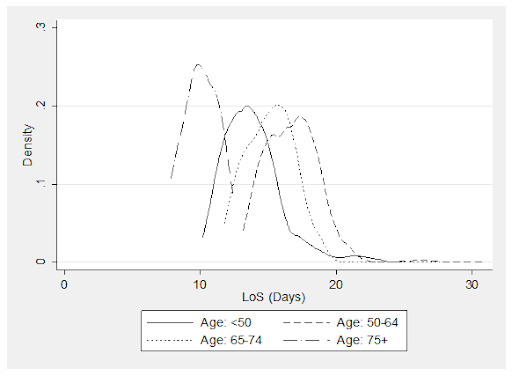
\includegraphics[width=\textwidth]{LOS_age.png}
    \caption{ Model-predicted LoS, by age group} \label{fig:fig1a}
    \end{subfigure}
\begin{subfigure}[b]{0.85\textwidth}
            \centering
            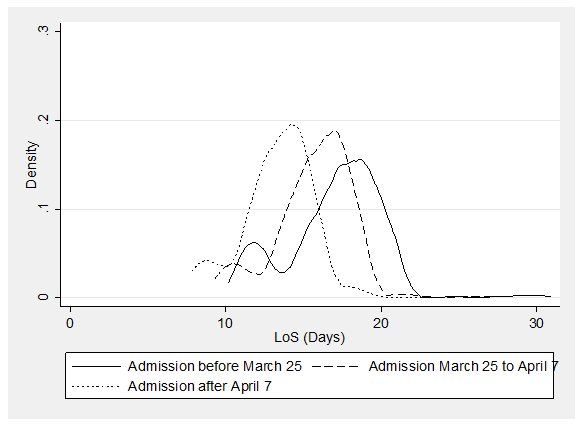
\includegraphics[width=\textwidth]{LOS_period.png}
    \caption{Model-predicted LoS, by admission period.}
    \label{fig:fig1b}
    \end{subfigure}
    \caption{\protect  Distribution of mean predicted LoS in ICU. Source: own elaboration using CHESS data.}
\end{figure}


Figure~\ref{fig:fig1a} shows that the age group with the shortest predicted mean LoS, 10.1 days (SD 1.2), was the oldest group (75 and older). Inspection of the final outcomes for this group showed that it was the one with the highest proportion of deaths (over 70\% of the non-censored cases). The next-shortest average LoS, of 13.8 days (SD 2.1) was for the youngest group (less than 50 years old). This younger group had the lowest proportion of deaths (less than 17\% of non-censored cases). The group with the longest predicted LoS was the 50-64 year old group, with a mean of 16.8 days (SD 2.0). 

Figure~\ref{fig:fig1b} shows a monotonic relationship between admission period and predicted LoS; the later the admission period, the shorter the LoS on average, with the early period having a mean predicted LoS of 17.1 days (SD 3.1) and the latest admission period, after April 7th, having a mean predicted LoS of 13.4 days (SD 2.2). The LoS distributions by admission period were notably bi-modal, with a small peak with relatively short LoS for each period. This was associated with the patients in the oldest age group, which, as shown in Figure 1a, had the shortest average predicted LoS by some margin. 

The inclusion of ethnicity (based on a smaller sample size $n=2,393$) does not improve the model fit (AIC=6201.62 without ethnicity vs AIC=6202.38 with ethnicity). Moreover, the qualitative findings from the model without ethnicity variable are virtually the same as in the model without ethnicity but with the full sample size $n=2,902$ (see Table~\ref{Table:ethnicity_model}).

\section{Discussion}

Our estimated mean LoS for ICU patients was 15 days. As expected, this was notably longer than the non-adjusted findings of ICNARC for England (2020; 12 days for survivors, 9 for non-survivors). Comparisons with other countries are less informative, because of differences in the populations and health-care systems, but our estimated LoS were longer than \cite{grasselli2020critical} for Italy, (2020; median 9 days), and \cite{Rees2020.04.30.20084780} 
for China (median of 8 days based on a compilation of 46 different studies); some studies reported median LoS in ICU as short as 5 days \citep{thomas2020coronavirus,wang2020clinical}.  

We found that ICU LoS was decreasing over our study period, with patients admitted before 25 March having LoS more than five days longer on average than those admitted after 7 April. There was no evidence of any differentiation of this effect between patients in various age groups, or with pre-existing risk factors. Unfortunately, the reasons for this change cannot be determined uniquely from our data, as several different and likely influential processes were confounded (except patient age, which we adjusted for): changes in the characteristics of patients contracting Covid-19 because of the stage of the epidemic, changes in who was admitted to ICU because of guideline changes, and changes over time in the treatment and management of Covid-19 patients. The first of the above possible explanations is further obscured by the non-uniform spread of the Covid-19 in regions of England, with London and the Midlands being hit first. The guidelines changes are likely to have a rather minor effect as the final decisions on whether to elevate care to intensive are ultimately taken by clinicians. Further, at no point, the capacity of the ICUs in England was overwhelmed by the number of patient, according to the NHS data on bed availability and occupancy~\cite{nhs2020}. However, some of the hospitals (e.g. in London) were closed to the limit.

It is not clear from our data whether this trend in shortening ICU LoS for Covid-19 patients was approaching an asymptote, but the balance among the influences on LoS may shift as the pandemic moves on from the first peak, possibly lengthening the LoS again in future waves of the pandemic.  

We found that the relationship between age and ICU LoS was not monotonic, unlike the relationship between age and Covid-19 severity and mortality~\cite{072020icnarc}. While the group with the shortest LoS was the oldest one, the group with the longest LoS was the “younger” middle-aged group between 50 and 64 years. The middle-aged groups in our sample tended to have a more even balance between those who died and those who recovered (for the patients with non-censored outcomes), i.e. the final outcome for these patients was likely the most uncertain on admission to ICU. 

We argue that the median LoS better describes the average LoS, but mean LoS might be better fit to be used in planning of the ICU capacity. In our case, mean LoS is five days longer than median (Table~\ref{Table:LOS_estimates_main}); this reveals that some of the Covid-19 patients tend to have very long LoS. This ought to be taken into account in situations when the infections are increasing exponentially during early phases of the pandemic or potential further waves. 

\subsection{Limitations}

%(just England, just the first peak, limited controls, much confounding, much missingness).

The CHESS data, while in principle being a census of all patients with Covid-19 in England, have severe missingness of cases. For example, when compared with the NHS Situation Reports (SitRep) deaths, they capture only around 13\% of deaths in hospitals. Those reported cases suffer from missingness of predictors, especially dates of admission to ICU and final outcome. The missingness patterns are also correlated with NHS trusts and geographies; London and the Midlands have highest percentages of missingness which might be due to these regions experiencing the peaks of the pandemic earlier than elsewhere. Further, each NHS trust operates their IT system autonomously, which may lead to discrepancies in coverage and quality of collecting non-routine data, such as individual-level CHESS data. These data-collection systems might have been under various levels of pressure during the peak of the pandemic.

Although our statistical models were suitable for adjusting the observed overall LoS for censoring, they are likely to be less useful for determining the potential causes of variation in LoS. This is because the overall LoS consists of sub-outcomes, i.e. death and recovery/discharge. The effect of risk-factors/predictors on these sub-outcomes may be countervailing, e.g. poor health state may predict a shorter LoS for eventual death but a longer LoS for eventual recovery. Our simple AFT models capture only the net effect of these predictors, and are not suitable for modelling these non-independent “competing” risks. More sophisticated models, such as competing risk AFT~\cite{lee2013nonparametric} and multistate models~\cite{putter2011}, that can account for such factors will allow for a more fine-grained analysis of the influences on ICU LoS (e.g. OUR COMPARISION PAPER REF).


%OLD (Before July 5th) Results section

%are negative, showing that all groups had lower  of a one-unit that LoS in ICU was associated significantly with the age group of the patient; those aged less than 50 (<50) had mean LoS only 80% as exp(-0.22)=0.8 or 80% of the reference group 50-64 LOS. For the oldest age group (75+), LOS is only 60% of the reference category. ECMO patients (N=79) have mean LOS around 50% longer (exp(0.4)=1.5). 

%The variable capturing temporal effect is also associated with the LOS: those admitted in the period prior to 25 March and between 25 March and 7 April 2020 have the ICU LOS 26% and 18% longer, respectively, compared with the admission to ICU after 7 April. 

%We do not find evidence of an association between sex of a patient and LOS in ICU, and inconsistent evidence of association with risk factors scores.

%In Table 2 we present details of the goodness-of-fit, including Akaike and Schwartz Bayesian Information Criteria (AIC and BIC) for the models under study. We find that models with both Weibull and log-normal distributions assumed for baseline hazards with the main effects only are better fit and thus chosen, with the-lognormal performing slightly better than Weibull. 

%The models consistently showed no association between the admission timing and specific age groups (interaction terms between age and ICU admission period, Table xxxx), nor the level of risk factors of patients with specific risk factors (interaction term between risk factor score and ICU admission period, Table xxxx). 

%\begin{table}[ht]
%\centering
%\caption{AIC and BIC for each parametric model. %Note: lower information criterion denotes a better %fitting model. \label{Tab:Table2}}
%\begin{tabular}[t]{lcccccc}
%\toprule
%	&	N	&	LL(null)	&	LL(model)	&	df	%&	AIC	&	BIC	\\
%\midrule

%Weibull - Main effects	&	2902	&	-3813.702&	%-3744.421&	10	&	7508.843&	7568.574	\\
%Weibull-Interactions	&	2902	&	-3813.702&	%-3741.826	&	18	&	7519.653	&	7627.169 \\
%Lognormal - Main effects	&	2902	&	%-3807.633	&	-3741.217	&	10	&	7502.434 &	%7562.166	\\
%Lognormal - Interactions	&	2902	&	%-3807.633 &	-3739.98 	&	18	&	7515.961 &	%7623.477	\\
%\bottomrule
%\end{tabular}
%\end{table}%



%\subsection{Interpretation of model coefficients}

%Based on the best-performing model, we find evidence that the 
%Length of Stay

%In Table xx2 we present the characteristics of predicted average mean and median LOS in ICU, disaggregated by age and period of admission to ICU. To calculate the average mean and median we first predict mean and median LOS for each individual in the sample and assuming a log-normal distribution for LOS \footnote{ Mean of log-normal distribution is given by exp(m + s2/2); median is exp(m), where m is the location and s is scale parameter of the distribution. }, and then calculate mean and standard deviation of the resulting two distributions: of individual means and individual medians. 

%The  predicted mean LOS is 15.0 days (SD=2.8) whereas predicted median is 10.1 (SD=1.9), which suggests that the distribution of means is right-skewed. We present the distributions in Figures … [figures from Maria]. The key feature of the distributions by age is that they are skewed and bimodal (why???). 

%Next, we present the means as they better capture possible long stays in ICU and may be more suitable for planning for the “worst case scenarios” in managing the demand for beds. The results by period of admission show the longest LOS in the period prior to 25 March (mean 17.1 days, SD=3.1), and the shortest after 7 April (mean=13.4, SD=2.2). This trend is consistent across all age groups. 

%The differences between age groups also reveal a pattern of the longest stays of patients aged 50-64 with mean=16.8 (SD=2.0), followed by 65-74 with mean 15.1 days (SD=1.7), <50 (mean=13.8, SD=2.1) and 75+ (mean=10.1, SD=1.2). The largest variability of the LOS (measured by SD) is proportional to the mean LOS by age and is decreasing with the period of admission for all age groups except for the youngest (<50), for which it is increasing with the period of admission (from SD=1.4 before 25 March to SD=2.1 after 7 April). 

%Finally, the distribution of mean and median LOS for ECMO patients is shown in Figure [ecmo LOS - appendix]

%\subsection{The effect of ethnicity}


%The two models below are the chosen model from before with only the cases with non-missing ethnicity (N=2393) and the model with five categories of ethnicity. The inclusion of ethnicity does not improve the model fit (AIC=6201.62 without ethnicity vs AIC=6202.38 with ethnicity). Moreover, the qualitative findings from the model without ethnicity variable are virtually the same as in the model without ethnicity but with the full sample size N=2902 (see Figure [ethnicity vs no ethnicity- appendix]. 

%\begin{table}[ht]
%\centering
%\caption{Log-normal model results: models with main effects (LHS) and model with interactions (RHS) %\label{Tab:Table3}}
%\begin{tabular}{lcccc}
%\hline
%\multicolumn{2}{c}{Log-Normal} \\
%\cline{2-5}
%	&	Coefficient	&	Robust SE	&	$z$	&	%$p>|z|$	\\
%\midrule
%female	&	-0.06	&	0.04	&	-1.42	&	%0.156	\\
% 	&		&		&		&		\\
%Admission Period (Ref: after April 7	&		&	%	&		&		\\
%Before March 25	&	0.28	&	0.06	&	4.28	%&	$<0.001$	\\
%March 25 - April 7	&	0.16	&	0.05	&	3.58	%&	$<0.001$	\\
%	&		&		&		&		\\
%Age (ref: 50-65)	&		&		&		&		%\\
%$<50$	&	-0.22	&	0.06	&	-3.8	&	%$<0.00$1	\\
%$65-74$	&	-0.11	&	0.05	&	-2.14	&	%0.033	\\
% $75+$	&	-0.52	&	0.06	&	-8.94	&	%$<0.001$	\\
% 	&		&		&		&		\\
%$risk_c$	&	-0.02	&	0.01	&	-1.42	&	%0.156	\\
% ecmo	&	0.4	&	0.14	&	2.85	&	0.004	%\\
% $_cons$	&	2.31	&	0.06	&	40.01	&	%$<0.001$	\\
%\bottomrule
%\end{tabular}
%\end{table}%


%\begin{center}
% TABLE HERE
%Table 3 Log-normal model results: models with main effects (LHS) and model with interactions (RHS)
%\end{center}

%\begin{table}[ht]
%\centering
%\caption{CAPTION \label{Tab:Table3}}
%\begin{tabular}[t]{lccccc}
%\toprule
%$<50$	&	mean	&	15.8	&	14.4	&	12.7	%&	13.8	\\
%	&	SD	&	1.4	&	1.7	&	2.1	&	2.1	\\
%	&	N	&	77	&	300	&	282	&	659	\\
%$50-64$	&	mean	&	19.7	&	17.5	&	%14.9	&	16.8	\\
%	&	SD	&	1.8	&	1.2	&	0.9	&	2	\\
%	&	N	&	136	&	631	&	478	&	1,245	\\
%$65-74$	&	mean	&	17.7	&	15.7	&	%13.2	&	15.1	\\
%	&	SD	&	1.2	&	0.6	&	0.5	&	1.7	\\
%	&	N	&	104	&	352	&	232	&	688	\\
%$75+$	&	mean	&	11.8	&	10.5	&	8.8	%&	10.1	\\
%	&	SD	&	0.5	&	0.4	&	0.3	&	1.2	\\
%	&	N	&	60	&	136	&	114	&	310	\\
%\bottomrule	
%Total	&	mean	&	17.1	&	15.7	&	13.4	%&	15	\\
%	&	SD	&	3.1	&	2.4	&	2.2	&	2.8	\\
%	&	N	&	377	&	1,419	&	1,106	&	%2,902	\\
%\bottomrule
%\end{tabular}
%\end{table}%

%\begin{figure}[h]
%\centering
%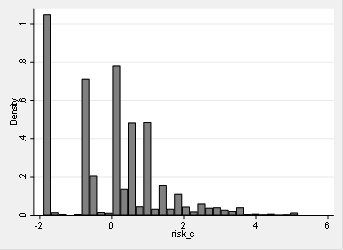
\includegraphics[width=0.5\textwidth]{risk_score.png}
%\caption{Risk Score \label{fig:fig4}}
%\end{figure}

%\begin{figure}[h]
%\centering
%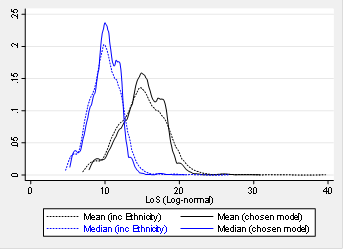
\includegraphics[width=0.5\textwidth]{LOS_ethnicity.png}
%\caption{Risk Score \label{fig:fig4}}
%\end{figure}


%\section{Limitations}

%Future/ongoing work

% \subsection{Conclusions}


\section*{Conflict of Interest statement}
All authors declare no conflict of interest.

\section*{Financial Disclosure statement}
The study has not been supported by any funding.


\newpage 

\appendix
\section{Appendix A: Data protocol}
\label{appendix:A} 

\subsection{Data preparation}

We use data from CHESS case records reported on 26 May 2020 with $N = 16,138$ entries. There were 15,750 with unique ID cases. The cases with identical IDs and with more than one entry were examined, and the following actions were taken:

\begin{enumerate}
\item When there were identical values for ICU admission date, but the entries had different hospital admission dates, the record with the earliest hospital admission date was kept.
\item When there were identical values for ICU admission date, but the entries had the same hospital admission dates, the record with the earliest swab date was kept.
\item When there were different values for ICU admission date and the ICU periods were not contiguous, all the entries were kept
\item When there were different values for the ICU admission date and the ICU periods were contiguous, a unique case was created based on the earliest hospital and ICU admission dates and the latest date of leaving ICU.
\item When any of the cases does not have an ICU admission date, the record with a non-missing value in this item was kept.
\item When any of the cases had an ICU admission date, but had different hospital admission dates, the record with the earliest date in the last item was kept.
\item When any of the cases had an ICU admission date, but had identical hospital admission dates, the record with the earliest swab date was kept.
 \end{enumerate}



Amongst the cases with different IDs and with only one entry, we found records with identical values in the hospital and ICU admission dates (date, hours and minutes), sex, age (year and month), trustcode and postcode. Given these coincidences, we only kept the record with the earliest estimated date of onset symptoms or swab date. After the deduplication process, 493 records were removed from the initial dataset.

In addition, the deduplicated dataset was filtered out by records whose hospital admission date was before 16 March 2020 (beginning of week 12) and after 24 May 2020 (end of week 21) ($n = 917$). Data before week 12 was excluded, given that the sample size was not enough for the current analysis ($n = 890$). Data after week 21 was omitted due to a lag of registering the complete information of each case. Therefore, we consider that the information of the most recent entries is unreliable.

Furthermore, the records which had missing values or unknown sex, negative values in age or recorded age of zero, and unavailable information regarding whether a patient was admitted to ICU or not led to a dataset of 13337 records.

From the 13,337 records, we removed 2,564 additional entries (Table~\ref{Tab:Trusts_removed}) These registers were reported by trusts where missigness is high.

\begin{table}
\centering
\small
\caption{Trusts removed from the analysis and respective number of deleted records.}
\label{Tab:Trusts_removed}
%\begin{tabular}[t]{lccc} 
% \setstretch{1}
\singlespacing
\begin{tabularx}{\textwidth}{>{\arraybackslash}m{3.5cm}ccc} 
\toprule
Trust name	&	Trust code	&	NHS region	&	Number of 	\\
	&	 	&		&	removed records\\ [2ex] \midrule
Basildon and Thurrock University Hospital	&	RDD	&	East of England	&	508	\\
Barking Havering and Redbridge University	&	RF4	&	London	&	426	\\
St George's Healthcare NHS Foundation	&	RJ7	&	London	&	102	\\
Imperial College Healthcare NHS Trust	&	RYJ	&	London	&	76	\\
The Hillingdon Hospitals Nhs Foundation	&	RAS	&	London	&	10	\\
Northampton General Hospital NHS Trust	&	RNS	&	Midlands	&	107	\\
Shrewsbury and Telford Hospital NHS Trust	&	RXW	&	Midlands	&	339	\\
University Hospitals Birmingham NHS Foundation	&	RRK	&	Midlands	&	3	\\
The Royal Orthopaedic Hospital NHS Foundation	&	RRJ	&	Midlands	&	39	\\
Wrightington Wigan and Leigh NHS Foundation	&	RRF	&	North West	&	498	\\
Bolton NHS Foundation Trust	&	RMC	&	North West	&	429	\\
East Kent Hospitals University NHS Foundation	&	RVV	&	South East	&	27	\\
\bottomrule
Total	&		&		&	2564	\\ 
\bottomrule
\end{tabularx}
%\end{tabular}
\end{table}%

\paragraph{Assumptions of LoS variable}

When the date of leaving ICU was the same as the final outcome date, it was assumed that an individual either died in ICU or was discharged from ICU. The date of censoring was either the date of last update of the record, or the swab date, which is the filtering used in the resulting analytical sample size. All negative LoS were removed from the analysis.

\newpage


\section{Descriptive statistics of LoS from ICU admission to leaving ICU} 

\begin{figure}[!ht]
    \centering
    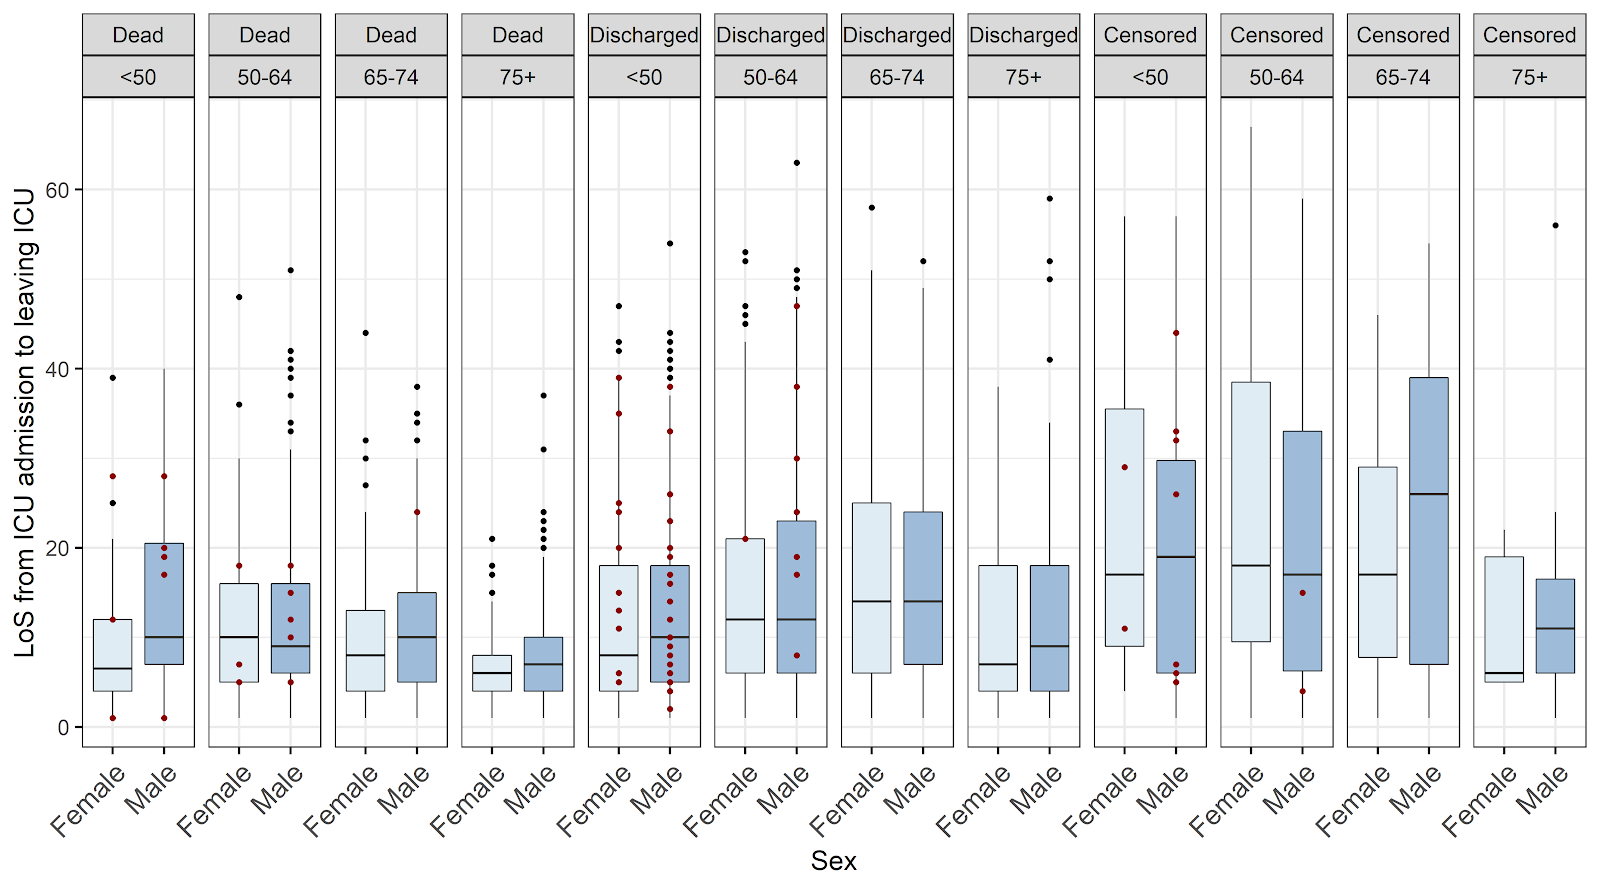
\includegraphics[width=0.95\textwidth]{LOS_descr_ASO.png}
    \caption{LoS from ICU admission to leaving ICU  by final outcome, sex and age of patients. Note: red dots denote ECMO patients. Last date of record update or swab date used for censoring. Source: own elaboration using CHESS data.}
    \label{Figure:los_desc_aso}
\end{figure}
\begin{figure}[!hb]
    \centering
    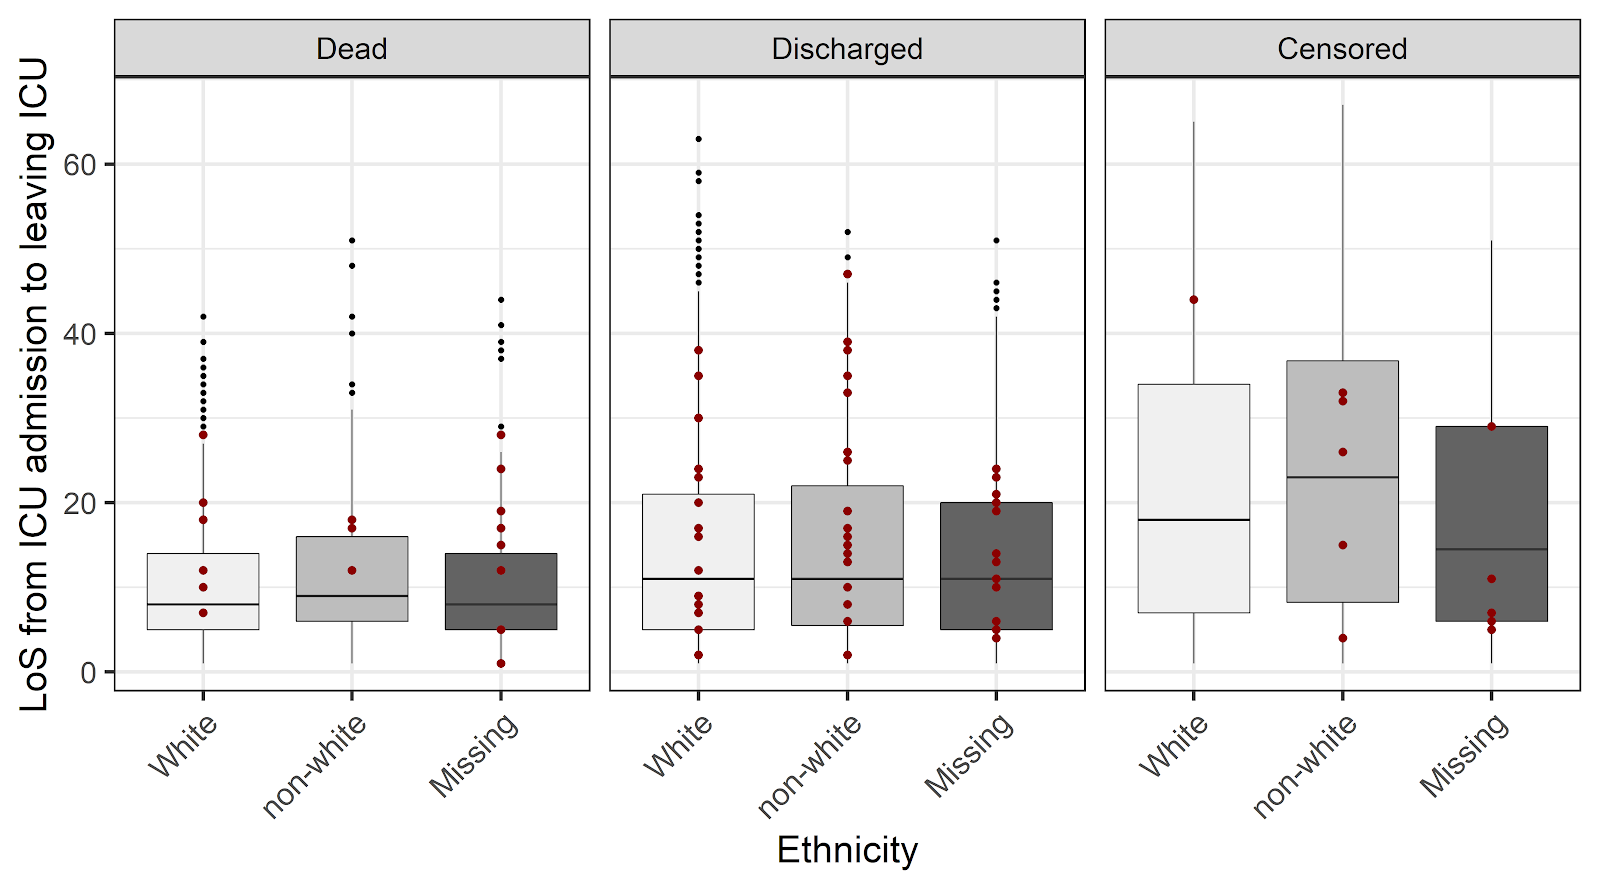
\includegraphics[width=0.95\textwidth]{LOS_descr_EthO.png}
    \caption{LoS from ICU admission to leaving ICU  by final outcome  and ethnicity of patients. Note: red dots denote ECMO patients. Last date of record update or swab date used for censoring. Source: own elaboration using CHESS data.}
    \label{Figure:los_desc_eth}
\end{figure}

\begin{landscape}
\begin{table}[htb]
  \centering\small
  \caption{Descriptive statistics of LoS from ICU admission to leaving ICU. Last date of record update or swab date were assumed for censoring.}
  \renewcommand{\arraystretch}{0.9}
  \setstretch{0.8}
    \begin{tabular}{cc|rrrrrr|rrrrrr}
    \toprule
    \multicolumn{2}{c|}{\textbf{Final outcome}} & \multicolumn{6}{c|}{\textbf{Death or discharged}} & \multicolumn{6}{c}{\textbf{Censored}} \\
    \midrule
    \textbf{Variable} & \textbf{Category} & \multicolumn{1}{c}{\textbf{Total}} & \multicolumn{1}{c}{\textbf{Mean}} & \multicolumn{1}{c}{\textbf{SD}} & \multicolumn{1}{c}{\textbf{Median}} & \multicolumn{1}{c}{\textbf{Min}} & \multicolumn{1}{c|}{\textbf{Max}} & \multicolumn{1}{c}{\textbf{Total}} & \multicolumn{1}{c}{\textbf{Mean}} & \multicolumn{1}{c}{\textbf{SD}} & \multicolumn{1}{c}{\textbf{Median}} & \multicolumn{1}{c}{\textbf{Min}} & \multicolumn{1}{c}{\textbf{Max}} \\
    \midrule
    \multicolumn{1}{c}{\multirow{2}{0.11\textwidth}{\textit{Sex}}} & \multicolumn{1}{l|}{Female} & 976   & 12.3  & 9.8   & 9     & 1     & 58    & 103   & 22.6  & 16.7  & 17    & 1     & 67 \\
          & \multicolumn{1}{l|}{Male} & 2278  & 12.9  & 10.2  & 10    & 1     & 63    & 246   & 20.9  & 15.5  & 18    & 1     & 59 \\
    \midrule
    \multicolumn{1}{c}{\multirow{4}[t]{0.11\textwidth}{\textit{Age groups}}} & \multicolumn{1}{l|}{$<$50} & 729   & 12.6  & 10.2  & 9     & 1     & 54    & 71    & 21.3  & 15.6  & 19    & 1     & 57 \\
          & \multicolumn{1}{l|}{50-64} & 1349  & 13.8  & 10.4  & 10    & 1     & 63    & 189   & 22.0  & 16.2  & 18    & 1     & 67 \\
          & \multicolumn{1}{l|}{65-74} & 801   & 12.8  & 9.7   & 10    & 1     & 58    & 69    & 22.3  & 15.9  & 19    & 1     & 54 \\
          & \multicolumn{1}{l|}{$>$75} & 375   & 9.0   & 8.1   & 7     & 1     & 59    & 20    & 13.3  & 12.3  & 11    & 1     & 56 \\
    \midrule
    \multicolumn{1}{c}{\multirow{3}[2]{0.11\textwidth}{\textit{Ethnicity}}} & \multicolumn{1}{l|}{White} & 1826  & 12.6  & 10.1  & 9     & 1     & 63    & 183   & 21.5  & 15.9  & 18    & 1     & 65 \\
          & \multicolumn{1}{l|}{Non-white} & 711   & 13.5  & 10.6  & 10    & 1     & 52    & 90    & 23.5  & 16.6  & 23    & 1     & 67 \\
          & \multicolumn{1}{l|}{Missing} & 717   & 12.3  & 9.3   & 10    & 1     & 51    & 76    & 18.6  & 14.6  & 15    & 1     & 51 \\
    \midrule
    \multicolumn{1}{c}{\multirow{5}[t]{0.11\textwidth}{\textit{Rash scores}}} & \multicolumn{1}{l|}{$<= -2.67$} & 893   & 12.5  & 10.0  & 9     & 1     & 63    & 95    & 21.5  & 15.5  & 17    & 1     & 67 \\
          & \multicolumn{1}{l|}{$(-2.67, -1.91]$} & 486   & 13.2  & 10.7  & 10    & 1     & 58    & 56    & 23.2  & 16.2  & 24    & 1     & 52 \\
          & \multicolumn{1}{l|}{$(-1.91, -1.03]$} & 519   & 13.2  & 10.2  & 10    & 1     & 59    & 53    & 22.0  & 16.5  & 18    & 1     & 57 \\
          & \multicolumn{1}{l|}{$> -1.03$} & 511   & 12.7  & 10.0  & 10    & 1     & 52    & 59    & 21.3  & 16.9  & 17    & 1     & 59 \\
          & \multicolumn{1}{l|}{Missing} & 845   & 12.4  & 9.6   & 9     & 1     & 53    & 86    & 19.7  & 15.1  & 17    & 1     & 65 \\
    \midrule
    \multicolumn{1}{c}{\multirow{2}[1]{0.11\textwidth}{\textit{ECMO patients}}} & \multicolumn{1}{l|}{Yes} & 68    & 16.9  & 10.6  & 16    & 1     & 47    & 11    & 19.3  & 14.0  & 15    & 4     & 44 \\
          & \multicolumn{1}{l|}{Missing} & 3186  & 12.6  & 10.0  & 10    & 1     & 63    & 338   & 21.5  & 15.9  & 18    & 1     & 67 \\
    \midrule
    \multicolumn{1}{c}{\multirow{3}[t]{0.11\textwidth}{\textit{ICU admission}}} & \multicolumn{1}{l|}{$<$25/03} & 436   & 14.1  & 11.2  & 10    & 1     & 63    & 32    & 27.8  & 21.5  & 22    & 2     & 67 \\
          & \multicolumn{1}{l|}{25/03 - 07/04} & 1650  & 13.5  & 10.4  & 10    & 1     & 59    & 105   & 27.7  & 17.3  & 28    & 1     & 59 \\
          & \multicolumn{1}{l|}{$>$ 07/04} & 1168  & 11.2  & 8.8   & 8     & 1     & 47    & 212   & 17.3  & 12.6  & 15    & 1     & 47 \\
    \midrule
    \multicolumn{1}{c}{\multirow{5}[t]{0.11\textwidth}{\textit{Hospital admission week}}} & \multicolumn{1}{l|}{12 or 13} & 1038  & 14.0  & 10.9  & 10    & 1     & 63    & 74    & 26.1  & 20.2  & 21    & 1     & 67 \\
          & \multicolumn{1}{l|}{14 or 15} & 1533  & 13.0  & 10.1  & 10    & 1     & 53    & 125   & 26.5  & 14.9  & 28    & 1     & 54 \\
          & \multicolumn{1}{l|}{16 or 17} & 476   & 11.6  & 8.6   & 9     & 1     & 40    & 77    & 20.5  & 11.9  & 22    & 1     & 42 \\
          & \multicolumn{1}{l|}{18 or 19} & 165   & 7.7   & 5.0   & 7     & 1     & 23    & 46    & 11.5  & 6.6   & 12    & 1     & 27 \\
          & \multicolumn{1}{l|}{20 or 21} & 42    & 3.9   & 2.5   & 4     & 1     & 12    & 27    & 4.3   & 3.4   & 3     & 1     & 13 \\
    \midrule
    \multicolumn{1}{c}{\multirow{7}[2]{0.11\textwidth}{\textit{Region}}} & \multicolumn{1}{l|}{London} & 535   & 14.5  & 11.3  & 11    & 1     & 54    & 43    & 28.5  & 17.5  & 26    & 1     & 67 \\
          & \multicolumn{1}{l|}{South East} & 484   & 12.3  & 9.6   & 9     & 1     & 63    & 61    & 21.3  & 16.6  & 17.0  & 1     & 65 \\
          & \multicolumn{1}{l|}{South West} & 294   & 13.3  & 10.9  & 9     & 1     & 59    & 20    & 16.5  & 12.6  & 16.5  & 1     & 41 \\
          & \multicolumn{1}{l|}{East} & 308   & 12.3  & 10.0  & 9     & 1     & 52    & 46    & 16.9  & 15.1  & 11.5  & 1     & 51 \\
          & \multicolumn{1}{l|}{Midlands} & 545   & 13.6  & 9.7   & 11    & 1     & 53    & 61    & 21.5  & 15.5  & 17    & 1     & 54 \\
          & \multicolumn{1}{l|}{North East \& Yorks} & 657   & 11.1  & 8.8   & 8     & 1     & 48    & 60    & 20.8  & 13.9  & 19    & 1     & 52 \\
          & \multicolumn{1}{l|}{North West} & 431   & 12.2  & 10.2  & 9     & 1     & 58    & 58    & 21.9  & 16.5  & 18    & 1     & 57 \\
    \midrule
    \multicolumn{2}{c|}{\textbf{Total}} & 3254  & 12.7  & 10.1  & 10    & 1     & 63    & 349   & 21.4  & 15.9  & 18    & 1     & 67 \\
    \bottomrule
    \multicolumn{14}{l}{\scriptsize{Source: own elaboration using CHESS data.}}
    \end{tabular}%
  \label{tab:descriptives}%
\end{table}%
\end{landscape}

\newpage 

\section{Models with interactions and with ethnicity \label{sec:other_models}}

\begin{table}[htbp]
\caption{Weibull Accelerated Failure Time model with main effects \label{Table:main_model_weibull} }
\centering
\begin{tabular}{lrrrr}\toprule
Variable	&	Coefficient	&	Robust SE	&	z	&	$p>|z|$	\\\midrule
     female	&	-0.05	&	0.04	&	-1.37	&	0.17	\\
           									
period	&	\multicolumn{4}{l}{(reference: after 07/04)}							\\
before 25/03	&	0.23	&	0.06	&	3.82	&	0	\\
25/03-07/04	&	0.16	&	0.04	&	4.12	&	0	\\
									\\
age group	&	\multicolumn{4}{l}{(reference: 50-64)}							\\
       $<50$ 	&	-0.16	&	0.06	&	-2.87	&	0	\\
     65-74 	&	-0.12	&	0.04	&	-2.75	&	0.033	\\
       $75+$ 	&	-0.50	&	0.06	&	-8.8	&	0	\\
risk score	&	-0.03	&	0.02	&	-1.98	&	0.156	\\
       ecmo	&	0.24	&	0.09	&	2.67	&	0.004	\\
intercept	&	2.72	&	0.05	&	51.02	&	0	\\\bottomrule
\end{tabular}
 \end{table}

\begin{table}[htp]
\caption{Log-normal and Weibull Accelerated Failure Time model with main and interaction effects   \label{Table:interactions_model} }
\centering
\begin{tabular}{lrrr|rrr}\toprule
& \multicolumn{3}{c}{Weibull}&\multicolumn{3}{c}{Log-normal}\\\midrule
variable	&	Coef.	&	Rob. SE	&	$P>|z|$	&		Coef.	&	Std. Err.	&	$P>|z|$	\\\toprule
ecmo	&	0.22	&	0.09	&	0.012	&		0.39	&	0.14	&	0.005	\\
female	&	-0.05	&	0.04	&	0.208	&		-0.06	&	0.04	&	0.155	\\
														
period	&	\multicolumn{6}{l}{(reference: after 07/04)}												\\
1	&	0.26	&	0.08	&	0.001	&		0.32	&	0.09	&	0.000	\\
2	&	0.13	&	0.06	&	0.017	&		0.15	&	0.07	&	0.027	\\
														
age group	&	\multicolumn{6}{l}{(reference: 50-64)}												\\
       $<50$ 	&	-0.14	&	0.08	&	0.062	&		-0.21	&	0.08	&	0.010	\\
     65-74 	&	-0.16	&	0.06	&	0.008	&		-0.13	&	0.08	&	0.083	\\
       $75+$ 	&	-0.54	&	0.09	&	0.000	&		-0.53	&	0.11	&	0.000	\\
														
\multicolumn{2}{l}{period*age group}			&		&		&			&		&		\\
1*$<50$	&	-0.11	&	0.10	&	0.292	&		-0.07	&	0.12	&	0.576	\\
1*65-74	&	0.03	&	0.12	&	0.823	&		-0.06	&	0.12	&	0.606	\\
1*$75+$	&	-0.07	&	0.17	&	0.655	&		-0.07	&	0.17	&	0.698	\\
2*$<50$	&	-0.02	&	0.11	&	0.877	&		-0.01	&	0.10	&	0.944	\\
2*65-74	&	0.08	&	0.08	&	0.307	&		0.06	&	0.09	&	0.517	\\
2*$75+$	&	0.11	&	0.14	&	0.440	&		0.05	&	0.14	&	0.725	\\
														
risk score	&	-0.02	&	0.02	&	0.409	&		-0.02	&	0.02	&	0.483	\\
														
\multicolumn{2}{l}{period*risk score}			&		&		&			&		&		\\
1	&	-0.05	&	0.04	&	0.219	&		-0.04	&	0.04	&	0.328	\\
2	&	-0.01	&	0.03	&	0.681	&		0.00	&	0.03	&	0.970	\\
														
intercept	&	2.73	&	0.06	&	0.000	&		2.32	&	0.07	&	0.000	\\\midrule
														
														
p	&	1.30	&	0.03	&0.000 & & &									\\
sigma	&		&		&		&		0.89	&	0.02	&0.000		\\\toprule
\multicolumn{7}{l}{\scriptsize{Note: Rob. SE denotes robust SE. Source: own elaboration using CHESS data.}}
\end{tabular}
 \end{table}

\begin{table}[htbp]
\caption{Predicted length-of-stay based on the log-normal model with main effects. \label{Table:LOS_estimates_main} }
\begin{center}
\begin{tabular}{llrrr|r}\toprule
Age	&	Measure	&	$<$25/03	&	25/03-07/04	&	$>$07/04	&	Total	\\\midrule
$<$50	&	mean	&	15.8	&	14.4	&	12.7	&	13.8	\\
	&	median	&	10.6	&	9.6	&	8.5	&	9.3	\\
	&	SD	&	1.4	&	1.7	&	2.1	&	2.1	\\
	&	N	&	77	&	300	&	282	&	659	\\

50-64	&	mean	&	19.7	&	17.5	&	14.9	&	16.8	\\
	&	median	&	13.2	&	11.8	&	10.0	&	11.2	\\
	&	SD	&	1.8	&	1.2	&	0.9	&	2.0	\\
	&	N	&	136	&	631	&	478	&	1,245	\\

65-74	&	mean	&	17.7	&	15.7	&	13.2	&	15.1	\\
	&	median	&	11.9	&	10.5	&	8.9	&	10.2	\\
	&	SD	&	1.2	&	0.6	&	0.5	&	1.7	\\
	&	N	&	104	&	352	&	232	&	688	\\

75+	&	mean	&	11.8	&	10.5	&	8.8	&	10.1	\\
	&	median	&	7.9	&	7.0	&	5.9	&	6.8	\\
	&	SD	&	0.5	&	0.4	&	0.3	&	1.2	\\
	&	N	&	60	&	136	&	114	&	310	\\\midrule

Total	&	mean	&	17.1	&	15.7	&	13.4	&	15.0	\\
	&	median	&	11.4	&	10.5	&	8.9	&	10.1	\\
	&	SD	&	3.1	&	2.4	&	2.2	&	2.8	\\
	&	N	&	377	&	1,419	&	1,106	&	2,902	\\\bottomrule
% 	\multicolumn{6}{l}{}
\end{tabular}
 \end{center}
 \scriptsize{Note: ``mean'' denotes a mean of the predicted mean LoS for all individual patients; ``median'' denotes a mean of the predicted median LoS for all patients. Source: own elaboration using CHESS data.}
 \end{table}

\begin{table}[htp]
\caption{Log-normal Accelerated Failure Time model with main effects results  \label{Table:ethnicity_model} }
\centering
\begin{tabular}{lrrr|rrr}\toprule
Variable	&	Coef.	&	Rob. SE	&			$p>|z|$	&	Coef.	&	Rob. SE	&			$p>|z|$	\\\toprule
     female	&	-0.06	&	0.05	&			0.257	&	-0.06	&	0.05	&			0.247	\\
           																	
period	&	\multicolumn{6}{l}{(reference: after 07/04)}															\\
before 25/03	&	0.33	&	0.07	&			0	&	0.33	&	0.07	&			0	\\
25/03-07/04	&	0.20	&	0.05	&			0	&	0.20	&	0.05	&			0	\\
																	
age group	&	\multicolumn{6}{l}{(reference: 50-64)}															\\
       $<50$ 	&	-0.22	&	0.07	&			0.002	&	-0.22	&	0.07	&			0.002	\\
     65-74 	&	-0.14	&	0.06	&			0.013	&	-0.14	&	0.05	&			0.01	\\
       $75+$ 	&	-0.54	&	0.06	&			0	&	-0.54	&	0.06	&			0	\\
risk score	&	-0.03	&	0.01	&			0.04	&	-0.03	&	0.01	&			0.028	\\
       ecmo	&	0.52	&	0.16	&			0.001	&	0.50	&	0.15	&			0.001	\\
																	
ethnicity	&	\multicolumn{6}{l}{(reference: White)}															\\
     Asian  	&		&		&				&	0.10	&	0.09	&			0.249	\\
     Black  	&		&		&				&	0.11	&	0.10	&			0.295	\\
     Mixed  	&		&		&				&	-0.13	&	0.17	&			0.43	\\
     Other  	&		&		&				&	-0.05	&	0.09	&			0.543	\\
intercept	&	2.30	&	0.06	&			0	&	2.28	&	0.06	&			0	\\\midrule
AIC	&	6201.62	&		&				&	6202.38	&		&				\\
N=2393& & & & & &\\\bottomrule

\multicolumn{7}{l}{Note: Rob SE denotes robust SE. Source: own elaboration using CHESS.}
\end{tabular}
 \end{table}


\newpage 

\bibliography{mybibfile}
%3850 without appendix
%4351 with
\end{document}